\documentclass[11pt]{article}

\usepackage{times}
\usepackage{amsfonts}
\usepackage{graphicx}
\usepackage{url,hyperref}
\usepackage{algonjk,tikz,latexsym,amsmath,amsthm}

\textheight 9.1in
\advance \topmargin by -1.0in
\textwidth 6.7in
\advance \oddsidemargin by -0.8in
\newcommand{\myparskip}{3pt}
\parskip \myparskip

\newtheorem{fact}{Fact}[section]
\newtheorem{lemma}{Lemma}[section]
\newtheorem{theorem}[lemma]{Theorem}
\newtheorem{assumption}[lemma]{Assumption}
\newtheorem{definition}[lemma]{Definition}
\newtheorem{corollary}[lemma]{Corollary}
\newtheorem{proposition}[lemma]{Proposition}
\newtheorem{claim}[lemma]{Claim}
\newtheorem{remark}[lemma]{Remark}
\newtheorem{prob}{Problem}
\newtheorem{conjecture}{Conjecture}

\renewcommand{\proofname}{\textbf{Proof}}
\newenvironment{proofof}[1]{\smallskip\noindent{\bf Proof of #1:}}{\hspace*{\fill}\par}


\newcommand{\etal}{{\em et al.}\ }
\newcommand{\assign}{\leftarrow}
\newcommand{\eps}{\epsilon}

\newcommand{\kec}[1]{-{\sc EC} }
\newcommand{\kvc}[1]{-{\sc VC} }
\newcommand{\ke}{\kec{2}}
\newcommand{\kv}{\kvc{2}}
\newcommand{\densV}{dens-{\sc VC} }
\newcommand{\densLP}{{\bf LP-dens} }

\newcommand{\ceil}[1]{\lceil #1 \rceil}
\newcommand{\floor}[1]{\lfloor #1 \rfloor}
\newcommand{\opt}{\textrm{\sc OPT}}
\newcommand{\lt}{\ell}

\newcommand{\len}[1]{length(#1) }
\newcommand{\weight}{w}
\newcommand{\dens}[1]{\emph{density}(#1)}
\DeclareMathAlphabet{\mathpzc}{OT1}{pzc}{m}{it}
\newcommand{\script}[1]{\mathcal{#1}}

\newcommand{\cR}{{\cal R}}

\bibliographystyle{plain}

\begin{document}

\title{Min-Cost -Connected Subgraphs With  Terminals}
\author{
  Chandra Chekuri\thanks{Dept. of Computer Science, University of Illinois, Urbana,
    IL 61801. Partially supported by NSF grants CCF 07-28782 and CNS-0721899, and a
    US-Israeli BSF grant 2002276. {\tt chekuri@cs.uiuc.edu}}
  \and 
  Nitish Korula\thanks{Dept. of Computer Science, University of Illinois, Urbana,
    IL 61801.  Partially supported by NSF grant CCF 07-28782. {\tt
      nkorula2@uiuc.edu}} }
\date{}
\maketitle

\begin{abstract}
  In the \kv problem, we are given an undirected graph  with edge
  costs and an integer ; the goal is to find a minimum-cost
  2-vertex-connected subgraph of  containing at least 
  vertices. A slightly more general version is obtained if the
  input also specifies a subset  of {\em terminals} and
  the goal is to find a subgraph containing at least  terminals.
  Closely related to the \kv problem, and in fact a special case of
  it, is the \ke problem, in which the goal is to find a minimum-cost
  2-edge-connected subgraph containing  vertices. The \ke problem
  was introduced by Lau \etal \cite{LauNSS07}, who also gave a
  poly-logarithmic approximation for it. No previous approximation
  algorithm was known for the more general \kv problem.  We describe
  an  approximation for the \kv problem.
\end{abstract}

\section{Introduction}
\label{sec:intro}

Connectivity and network design problems play an important role in
combinatorial optimization and algorithms both for their theoretical
appeal and their many real-world applications. An interesting and
large class of problems are of the following type: given a graph
 with edge or node costs, find a minimum-cost subgraph  of
 that satisfies certain connectivity properties. For example, given
an integer , one can ask for the minimum-cost spanning
subgraph that is -edge or -vertex connected. If
 then this is the classical minimum spanning tree (MST)
problem. For  the problem is NP-hard and also APX-hard to
approximate. More general versions of connectivity problems are
obtained if one seeks a subgraph in which a subset of the nodes  referred to as {\em terminals} are -connected.
The well-known Steiner tree problem is to find a minimum-cost subgraph
that (-)connects a given set . Many of these problems are
special cases of the survivable network design problem (SNDP). In
SNDP, each pair of nodes  specifies a connectivity
requirement  and the goal is to find a minimum-cost subgraph
that has  disjoint paths for each pair . Given the
intractability of these connectivity problems, there has been a large
amount of work on approximation algorithms. A number of elegant and
powerful techniques and results have been developed over the years
(see \cite{Hochbaum96,Vazirani01}). In particular, the primal-dual
method \cite{AgrawalKR95,GoemansW96} and iterated rounding \cite{Jain}
have led to some remarkable results including a -approximation for
edge-connectivity SNDP \cite{Jain}.

An interesting class of problems, related to some of the connectivity
problems described above, is obtained by requiring that only  of
the given terminals be connected. These problems are partly motivated
by applications in which one seeks to maximize profit given a upper
bound (budget) on the cost.  For example, a useful problem in vehicle
routing applications is to find a path that maximizes the number of
vertices in it subject to a budget  on the length of the path. In
the exact optimization setting, the profit maximization problem is
equivalent to the problem of minimizing the cost/length of a path
subject to the constraint that at least  vertices are included. Of
course the two versions need not be approximation equivalent,
nevertheless, understanding one is often fruitful or necessary to
understand the other. The most well-studied of these problems is the
-MST problem; the goal here is to find a minimum-cost subgraph of
the given graph  that contains at least  vertices (or
terminals). This problem has attracted considerable attention in the
approximation algorithms literature and its study has led to several
new algorithmic ideas and applications
\cite{AwerbuchABV95,Garg96,Garg05,ChaudhuriGRT03,orienteering}.  We
note that the Steiner tree problem can be relatively easily reduced in
an approximation preserving fashion to the -MST problem.  More
recently, Lau \etal \cite{LauNSS07} considered the natural
generalization of -MST to higher connectivity. In particular they
defined the -subgraph problem to be the following: find a
minimum-cost subgraph of the given graph  that contains at least
 vertices and is -edge connected. We use the notation
\kec{\lambda} to refer to this problem. In \cite{LauNSS07} an
 approximation was claimed for the \ke problem.  However,
the algorithm and proof in \cite{LauNSS07} are incorrect.  More
recently, and in independent work from ours, the authors of
\cite{LauNSS07} obtained a different algorithm for \ke that yields an
 approximation. We give later a more detailed comparison
between their approach and ours. It is also shown in \cite{LauNSS07}
that a good approximation for \kec{\lambda} when  is large
would yield an improved algorithm for the -densest subgraph problem
\cite{FeigeKP01}; in this problem one seeks a -vertex subgraph of a
given graph  that has the maximum number of edges. The -densest
subgraph problem admits an  approximation for some
fixed constant  \cite{FeigeKP01}, but has resisted
attempts at an improved approximation for a number of years now.

In this paper we consider the vertex-connectivity generalization of
the -MST problem. We define the \kvc{\lambda} problem as follows:
Given an integer  and a graph  with edge costs, find the
minimum-cost -vertex-connected subgraph of  that contains
at least  vertices. We also consider the {\em terminal} version of
the problem where the subgraph has to contain  terminals from a
given terminal set . It can be easily shown that the
\kec{\lambda} problem reduces to the \kvc{\lambda} problem for any . We also observe that the \kec{\lambda} problem with terminals
can be easily reduced, as follows, to the uniform problem where every
vertex is a terminal: For each terminal , create  dummy
vertices  and attach  to  with
 parallel edges of zero cost. Now set  in the new
graph. One can avoid using parallel edges by creating a clique on
 using zero-cost edges and connecting 
of these vertices to . Note, however, that this reduction only
works for edge-connectivity. We are not aware of a reduction that
reduces the \kvc{\lambda} problem with a given set of terminals to the
\kvc{\lambda} problem, even when . In this paper we
consider the \kv problem; our main result is the following.

\begin{theorem}
  \label{thm:kv}
  There is an  approximation for the \kv
  problem where  is the number of terminals.
\end{theorem}

\begin{corollary}
  \label{cor:ke}
  There is an  approximation for the \ke
  problem where  is the number of terminals.
\end{corollary}

One of the technical ingredients that we develop is the theorem below
which may be of independent interest. Given a graph  with edge costs
and weights on terminals , we define  for a
subgraph  to be the ratio of the cost of edges in  to the total
weight of terminals in .

\begin{theorem}
  \label{thm:cycle}
  Let  be an -vertex-connected graph with edge costs and let  be a set of terminals. Then, there is a simple cycle 
  containing at least  terminals (a non-trivial cycle) such that
  the density of  is at most the density of . Moreover, such a
  cycle can be found in polynomial time.
\end{theorem}

Using the above theorem and an LP approach we obtain the following. 
\begin{corollary}
  \label{cor:cycle}
  Given a graph  with edge costs and  terminals
  , there is an  approximation for the
  problem of finding a minimum-density non-trivial cycle.
\end{corollary}

Note that Theorem~\ref{thm:cycle} and Corollary~\ref{cor:cycle} are of
interest because we seek a cycle with at least {\em two} terminals.  A
minimum-density cycle containing only one terminal can be found by
using the well-known min-mean cycle algorithm in directed graphs
\cite{networkflows_book}.  We remark, however, that although we
suspect that the problem of finding a minimum-density non-trivial
cycle is NP-hard, we currently do not have a proof.
Theorem~\ref{thm:cycle} shows that the problem is equivalent to the
\densV problem, defined in the next section.

\smallskip
\noindent {\bf Remark:} The reader may wonder whether \ke or \kv admit
a constant factor approximation, since the -MST problem admits one.
We note that the main technical tool which underlies 
approximations for -MST problem \cite{BlumRV96,Garg96,ChudakRW} is
a special property that holds for a LP relaxation of the
prize-collection Steiner tree problem \cite{GoemansW96} which is a
Lagrangian relaxation of the Steiner tree problem. Such a property is
not known to hold for generalizations of -MST including \ke and \kv
and the -Steiner forest problem \cite{HajiaghayiJ}. Thus, one is
forced to rely on alternative and problem-specific techniques.


\subsection{Overview of Technical Ideas}
We consider the rooted version of \kv: the goal is to find a min-cost
subgraph that -connects at least  terminals to a specified root
vertex . It is relatively straightforward to reduce \kv to its
rooted version (see section~\ref{sec:k2vc} for details.)  We draw
inspiration from algorithmic ideas that led to poly-logarithmic
approximations for the -MST problem. 

To describe our approach to the rooted \kv problem, we define a
closely related problem. For a subgraph  that contains , let
 be the number of terminals that are -connected to  in
. Then the {\em density} of  is simply the ratio of the cost of
 to . The \densV problem is to find a 2-connected subgraph of
minimum density. An  approximation for the \densV
problem (where  is the number of terminals) can be derived in a
some what standard way by using a bucketing and scaling trick on a
linear programming relaxation for the problem. We exploit the known
bound of  on the integrality gap of a natural LP for the SNDP
problem with vertex connectivity requirements in 
\cite{FleischerJW}.  The bucketing and scaling trick has seen several
uses in the past and has recently been highlighted in several
applications \cite{ChekuriHKS06,ChekuriHKS07,ChekuriEGS08}.

Our algorithm for \kv uses a greedy approach at the high level. We
start with an empty subgraph  and use the approximation algorithm
for \densV in an iterative fashion to greedily add terminals to 
until at least  terminals are in . This approach would
yield an  approximation if . However,
the last iteration of the \densV algorithm may add many more terminals
than desired with the result that . In this case we cannot
bound the quality of the solution obtained by the algorithm.  To
overcome this problem, one can try to {\em prune} the subgraph 
added in the last iteration to only have the desired number of
terminals. For the -MST problem,  is a tree and pruning is
quite easy. We remark that this yields a rather straightforward
 approximation for -MST and could have been
discovered much before a more clever analysis given in
\cite{AwerbuchABV95}.

One of our technical contributions is to give a pruning step for the
\kv problem. To accomplish this, we use two algorithmic ideas. The
first is encapsulated in the cycle finding algorithm of
Theorem~\ref{thm:cycle}.  Second, we use this cycle finding algorithm
to repeatedly merge subgraphs until we get the desired number of
terminals in one subgraph. This latter step requires care. The cycle
merging scheme is inspired by a similar approach from the work of Lau
\etal \cite{LauNSS07} on the \ke problem and in \cite{ChekuriKP08} on
the directed orienteering problem. These ideas yield an  approximation. We give a slightly modified
cycle-merging algorithm with a more sophisticated and non-trivial
analysis to obtain an improved 
approximation.

Some remarks are in order to compare our work to that of
\cite{LauNSS07} on the \ke problem. The combinatorial algorithm in
\cite{LauNSS07} is based on finding a low-density
cycle or a related structure called a bi-cycle. The algorithm in
\cite{LauNSS07} to find such a structure is incorrect.  Further, the
cycles are contracted along the way which limits the approach to the
\ke problem (contracting a cycle in -node-connected graph may make
the resulting graph not -node-connected).  In our algorithm we do
not contract cycles and instead introduce dummy terminals with weights
to capture the number of terminals in an already formed component.
This requires us to now address the minimum-density non-trivial simple
cycle problem which we do via Theorem~\ref{thm:cycle} and
Corollary~\ref{cor:cycle}. In independent work, Lau \etal
\cite{LauNSS07b} obtain a new and correct -approximation for \ke.  They also follow the same approach that we
do in using the LP for finding dense subgraphs followed by the pruning
step.  However, in the pruning step they use a completely different
approach; they use the sophisticated idea of no-where zero -flows
\cite{Seymour}. Although the use of this idea is elegant, the approach
works only for the \ke problem, while our approach is less complex
and leads to an algorithm for the more general \kv problem.


\section{The Algorithm for the \kv Problem}\label{sec:k2vc}

We work with graphs in which some vertices are designated as
\emph{terminals}.  Given a graph  with edge costs and terminal
weights, we define the \emph{density} of a subgraph  to be sum of
the costs of edges in  divided by the sum of the weights of
terminals in .  Henceforth, we use -connected graph to mean a
-vertex-connected graph.

The goal of the \kv problem is to find a minimum-cost 2-connected
subgraph on at least  terminals.\footnote{In fact, our algorithm
  solves the harder problem in which terminals have weights, and the
  goal is to find a minimum-cost 2-connected subgraph in which the sum
  of terminal weights is at least . For simplicity of exposition,
  however, we stick to the more restricted version.}  Recall that in
the rooted \kv problem, the goal is to find a min-cost subgraph on at
least  terminals in which every terminal is 2-connected to the
specified root . The (unrooted) \kv problem can be reduced to the
rooted version by \emph{guessing} 2 vertices  that are in an
optimal solution, creating a new root vertex , and connecting it
with 0-cost edges to  and . It is not hard to show that any
solution to the rooted problem in the modified graph can be converted
to a solution to the unrooted problem by adding 2 minimum-cost
vertex-disjoint paths between  and .  (Since  and  are in
the optimal solution, the cost of these added paths cannot be more
than .) We omit further details from this extended abstract.

In the \densV problem, the goal is to find a subgraph  of minimum
density in which all terminals of  are 2-connected to the root. The
following lemma is proved in Section~\ref{subsec:LP} below.  It relies
on a -approximation, via a natural LP, for the min-cost
-connectivity problem due to Fleischer, Jain and Williamson
\cite{FleischerJW}, and some standard techniques.

\begin{lemma}\label{lem:densV}
  There is an -approximation algorithm for the \densV
  problem, where  is the number of terminals in the given
  instance.
\end{lemma}

Let  be the cost of an optimal solution to the \kv problem. We
assume knowledge of ; this can be dispensed with using standard
methods.  We pre-process the graph by deleting any terminal that does
not have 2 vertex-disjoint paths to the root  of total cost at most
. The high-level description of the algorithm for the 
rooted \kv problem is given below.

\begin{algo}
  ,  is the empty graph. \\
  While (): \+ \\
  Use the approximation algorithm for \densV to find a subgraph  in .\\
  If (): \+ \\
  ,  \\
  Mark all terminals in  as non-terminals. \- \\
  Else: \+ \\
  {\em Prune}  to obtain  that contains  terminals. \\
  ,  \- \- \\
  Output 
\end{algo}

At the beginning of any iteration of the while loop, the graph contains a
solution to the \densV problem of density at most .
Therefore, the graph  returned always has density at most . If , we add  to  and decrement ;
we refer to this as the \emph{augmentation} step. Otherwise, we have a
graph  of good density, but with too many terminals. In this case, we
prune  to find a graph with the required number of terminals; this is
the \emph{pruning step}. A simple set-cover type argument shows the
following lemma:

\begin{lemma}\label{lem:greedy}
  If, at every augmentation step, we add a graph of density at most
   (where  is the number of
  additional terminals that must be selected), the total cost of all
  the augmentation steps is at most .
\end{lemma}

Therefore, we now only have to bound the cost of the graph  added
in the pruning step; we prove the following theorem in
Section~\ref{sec:pruning}.

\begin{theorem} \label{thm:avekv} Let  be an
  instance of the rooted \kv problem with root , such that every
  vertex of  has  vertex-disjoint paths to  of total cost at
  most , and such that . There is a
  polynomial-time algorithm to find a solution to this instance of
  cost at most .
\end{theorem}

\noindent We can now prove our main result for the \kv problem,
Theorem~\ref{thm:kv}.

\begin{proofof}{Theorem~\ref{thm:kv}}
  Let  be the cost of an optimal solution to the (rooted) \kv
  problem.  By Lemma~\ref{lem:greedy}, the total cost of the
  augmentation steps of our greedy algorithm is . To bound the cost of the pruning step, let  be
  the number of additional terminals that must be covered just prior
  to this step. The algorithm for the \densV problem returns a graph
   with  terminals, and density at most . As a result of our pre-processing step, every
  vertex has 2 vertex-disjoint paths to  of total cost at most
  . Now, we use Theorem~\ref{thm:avekv} to prune  and find a
  graph  with  terminals and cost at most . Therefore, the total cost of our solution is .
\end{proofof}

\bigskip
It remains only to prove Lemma~\ref{lem:densV}, that there is an -approximation for the \densV problem, and
Theorem~\ref{thm:avekv}, bounding the cost of the pruning step. We
prove the former in Section~\ref{subsec:LP} below. Before the latter
is proved in Section~\ref{sec:pruning}, we develop some tools in
Section~\ref{sec:cycles}; chief among these tools is
Theorem~\ref{thm:cycle}. 

\subsection{An -approximation for the \densV problem}
\label{subsec:LP}

Recall that the \densV~problem was defined as follows: Given a graph
 with edge-costs, a set  of terminals, and a
root , find a subgraph  of minimum density, in which
every terminal of  is 2-connected to . (Here, the density of 
is defined as the cost of  divided by the number of terminals it
contains, not including .)  We describe an algorithm for \densV
that gives an -approximation, and sketch its proof. We
use an LP based approach and a bucketing and scaling trick (see
\cite{ChekuriEGS08,ChekuriHKS06,ChekuriHKS07} for applications of this
idea), and a constant-factor bound on the integrality gap of an LP for
SNDP with vertex-connectivity requirements in 
\cite{FleischerJW}.

\bigskip
We define \densLP as the following LP relaxation of \densV. For each
terminal , the variable  indicates whether or not  is
chosen in the solution. (By normalizing  to 1, and
minimizing the sum of edge costs, we minimize the density.)
 is the set of all simple cycles containing  and the
root ; for any ,  indicates how much
`flow' is sent from  to  through . (Note that a pair of
vertex-disjoint paths is a cycle; the flow along a cycle is 1 if we
can 2-connect  to  using the edges of the cycle.) The variable
 indicates whether the edge  is used by the solution.

\newpage

\vspace{-0.15in}


\vspace{-0.15in}
It is not hard to see that an optimal solution to \densLP has cost at
most the density of an optimal solution to \densV. We now show how to
obtain an integral solution of density at most , where  is the cost of an optimal solution to
\densLP.  The linear program \densLP has an exponential number of
variables but a polynomial number of non-trivial constraints; it can,
however, be solved in polynomial time. Fix an optimal solution to
\densLP of cost , and for each  (for
ease of notation, assume  is an integer), let  be the
set of terminals  such that . Since
, there is some index  such that . Since every terminal  has , the number of terminals in  is at
least .  We claim that there is a subgraph
 of  with cost at most , in which every
terminal of  is 2-connected to the root. If this is true, the
density of  is at most , and hence we
have an -approximation for the \densV problem.

To prove our claim about the cost of the subgraph  in which every
terminal of  is 2-connected to , consider scaling up the given
optimum solution of \densLP by a factor of . For each
terminal , the flow from  to  in this scaled
solution\footnote{This is an abuse of the term `solution', since after
  scaling, } is at least 1, and the cost
of the scaled solution is .

In \cite{FleischerJW}, the authors describe a linear program  to
find a minimum-cost subgraph in which a given set of terminals is
2-connected to the root, and show that this linear program has an
integrality gap of 2. The variables  in the `scaled solution' to
\densLP correspond to a feasible solution of  with  as the
set of terminals; the integrality gap of 2 implies that there is a
subgraph  in which every terminal of  is 2-connected to the
root, with cost at most .

Therefore, the algorithm for \densV is: 
\begin{enumerate}
  \item Find an optimal fractional solution to \densLP.

  \item Find a set of terminals  such that .

  \item Find a min-cost subgraph  in which every terminal in 
    is 2-connected to  using the algorithm of \cite{FleischerJW}.
     has density at most  times the optimal solution
    to \densV.
\end{enumerate}

\section{Finding Low-density Non-trivial Cycles}
\label{sec:cycles}

A cycle  is \emph{non-trivial} if it contains at least 2
terminals.  We define the min-density non-trivial cycle problem: Given a
graph , with  marked as terminals, edge costs and
terminal weights, find a minimum-density cycle that contains at least 2
terminals. Note that if we remove the requirement that the cycle be
non-trivial (that is, it contains at least 2 terminals), the problem
reduces to the min-mean cycle problem in directed graphs, and can be solved
exactly in polynomial time (see \cite{networkflows_book}).  Algorithms for
the min-density non-trivial cycle problem are a useful tool for solving the
\kv and \ke problems. In this section, we give an -approximation algorithm for the minimum-density non-trivial cycle
problem.

First, we prove Theorem~\ref{thm:cycle}, that a 2-connected graph with
edge costs and terminal weights contains a simple non-trivial cycle,
with density no more than the average density of the graph. We give
two algorithms to find such a cycle; the first, described in
Section~\ref{subsec:nonPoly}, is simpler, but the running time is not
polynomial.  A more technical proof that leads to a strongly
polynomial-time algorithm is described in Section~\ref{subsec:strong};
we recommend this proof be skipped on a first reading.

\subsection{An Algorithm to Find Cycles of Average
  Density}\label{subsec:nonPoly}

To find a non-trivial cycle of density at most that of the 2-connected
input graph , we will start with an arbitrary non-trivial cycle,
and successively find cycles of better density until we obtain a cycle
with density at most . The following lemma shows that if a
cycle  has an ear with density less than , we can use
this ear to find a cycle of lower density.

\begin{lemma}\label{lem:goodEar}
  Let  be a non-trivial cycle, and  an ear incident to  at
   and , such that . Let  and  be the two internally disjoint paths
  between  and  in . Then  and  are
  both simple cycles and one of these is non-trivial and has density
  less than .
\end{lemma}
\begin{proof}
   has at least 2 terminals, so it has finite density;  must
  then have at least 1 terminal. Let ,  and  be,
  respectively, the sum of the costs of the edges in ,  and
  , and let ,  and  be the sum of the weights of the
  terminals in ,  and .

  Assume w.l.o.g. that  has density at most that of . (That
  is, .)\footnote{It is possible that one of
     and  has cost 0 and weight 0. In this case, let 
    be the component with non-zero weight.}   must contain at
  least one terminal, and so  is a simple non-trivial
  cycle.  The statement  is equivalent
  to .
  \vspace{-0.2in}

  

  \vspace{-0.2in}
  Therefore,  is a simple cycle containing at least 2 terminals of
  density less than .
\end{proof}

\begin{lemma}\label{lem:2connComp}
  Given a cycle  in a -connected graph , let  be the graph
  formed from  by contracting  to a single vertex . If  is
  a connected component of ,  is -connected in
  .
\end{lemma}
\begin{proof}
  Let  be an arbitrary connected component of , and let . To prove that  is 2-connected, we first observe
  that  is 2-connected to any vertex . (Any set that
  separates  from  in  separates  from the cycle  in
  .)

  It now follows that for all vertices ,  and  are
  2-connected in . Suppose deleting some vertex  separates 
  from . The vertex  cannot be , since  is a connected
  component of . But if ,  and  are in the
  same component of , since  is 2-connected to  in
  . Similarly,  and  are in the same component of ,
  and so deleting  does not separate  from .
\end{proof}

We now show that given any 2-connected graph , we can find a
non-trivial cycle of density no more than that of .

\begin{theorem}\label{thm:cycleExists} 
  Let  be a -connected graph with at least  terminals. 
  contains a simple non-trivial cycle  such that .
\end{theorem}
\begin{proof}
  Let  be an arbitrary non-trivial simple cycle; such a cycle
  always exists since  is -connected and has at least 2
  terminals.  If , we give an algorithm that
  finds a new non-trivial cycle  such that .
  Repeating this process, we obtain cycles of successively better
  densities until eventually finding a non-trivial cycle  of
  density at most .

  Let  be the graph formed by contracting the given cycle  to a
  single vertex . In ,  is not a terminal, and so has weight
  0. Consider the 2-connected components of  (from
  Lemma~\ref{lem:2connComp}, each such component is formed by adding
   to a connected component of ), and pick the one of
  minimum density. If  is this component,  by
  an averaging argument.

   contains at least 1 terminal. If it contains 2 or more
  terminals, recursively find a non-trivial cycle  in  such
  that . If  exists in the
  given graph , it has the desired properties, and we are
  done. Otherwise,  contains , and the edges of  form a ear
  of  in the original graph . The density of this ear is less
  than the density of , so we can apply Lemma~\ref{lem:goodEar} to
  obtain a non-trivial cycle in  that has density less than
  .

  Finally, if  has exactly 1 terminal , find any 2
  vertex-disjoint paths using edges of  from  to distinct
  vertices in the cycle . (Since  is 2-connected, there always
  exist such paths.) The cost of these paths is at most , and
  concatenating these 2 paths corresponds to a ear of  in .  The
  density of this ear is less than ; again, we use
  Lemma~\ref{lem:goodEar} to obtain a cycle in  with the desired
  properties.
\end{proof}

We remark again that the algorithm of Theorem~\ref{thm:cycleExists} does
not lead to a polynomial-time algorithm, even if all edge costs and
terminal weights are polynomially bounded. In Section~\ref{subsec:strong},
we describe a strongly polynomial-time algorithm that, given a graph ,
finds a non-trivial cycle of density at most that of .
Note that neither of these algorithms may directly give a good
approximation to the min-density non-trivial cycle problem, because
the optimal non-trivial cycle may have density much less than that of
.  However, we can use Theorem~\ref{thm:cycleExists} to prove the
following theorem:

\begin{theorem}\label{thm:equivalence}
  There is an -approximation to the (unrooted) \densV problem
  if and only if there is an -approximation to the problem of
  finding a minimum-density non-trivial cycle.
\end{theorem}
\begin{proof}
  Assume we have a -approximation for the \densV
  problem; we use it to find a low-density non-trivial cycle. Solve
  the \densV problem on the given graph; since the optimal cycle is a
  2-connected graph, our solution  to the \densV problem has
  density at most  times the density of this cycle.
  Find a non-trivial cycle in  of density at most that of ; it
  has density at most  times that of an optimal
  non-trivial cycle.

  Note that any instance of the (unrooted) \densV problem has an
  optimal solution that is a non-trivial cycle.  (Consider any optimal
  solution  of density ; by Theorem~\ref{thm:cycle}, 
  contains a non-trivial cycle of density at most . This cycle
  is a valid solution to the \densV problem.) Therefore, a
  -approximation for the min-density non-trivial cycle
  problem gives a -approximation for the \densV problem.
\end{proof}

Theorem~\ref{thm:equivalence} and Lemma~\ref{lem:densV} imply 
an -approximation for the minimum-density non-trivial cycle
problem; this proves Corollary~\ref{cor:cycle}.

We say that a graph  is minimally 2-connected on its terminals
if for every edge , some pair of terminals is not 2-connected
in the graph .  Section~\ref{subsec:strong} shows that in any
graph which is minimally 2-connected on its terminals, every cycle is
non-trivial.  Therefore, the problem of finding a minimum-density
non-trivial cycle in such graphs is just that of finding a
minimum-density cycle, which can be solved exactly in polynomial
time. However, as we explain at the end of the section, this does not
directly lead to an efficient algorithm for arbitrary graphs.

\subsection{A Strongly Polynomial-time Algorithm to Find Cycles of Average
  Density}\label{subsec:strong}

In this section, we describe a strongly polynomial-time algorithm
which, given a 2-connected graph  with edge costs and terminal
weights, finds a non-trivial cycle of density at most that of .

We begin with several definitions: Let  be a cycle in a graph ,
and  be the graph formed by deleting  from . Let  be the connected components of ; we refer to these as
\emph{earrings} of .\footnote{If  were simply a path, it would be an
  ear of , but  may be more complex.}  For each , let the
vertices of  incident to it be called its \emph{clasps}. From the
definition of an earring, for any pair of clasps of , there is a
path between them whose internal vertices are all in . 

We say that a vertex of  is an \emph{anchor} if it is the clasp of
some earring. (An anchor may be a clasp of multiple earrings.)  A
\emph{segment}  of  is a path contained in , such that the
endpoints of  are both anchors, and no internal vertex of  is an
anchor. (Note that the endpoints of  might be clasps of the same
earring, or of distinct earrings.) It is easy to see that the segments
partition the edge set of . By deleting a segment, we refer to
deleting its edges and internal vertices. Observe that if  is
deleted from , the only vertices of  that lose an edge are
the endpoints of . A segment is \emph{safe} if the graph  is
2-connected.

Arbitrarily pick a vertex  of  as the \emph{origin}, and
consecutively number the vertices of  clockwise around the cycle as
. The first clasp of an earring
 is its lowest numbered clasp, and the last clasp is its highest
numbered clasp. (If the origin is a clasp of , it is considered the
first clasp, not the last.) The \emph{arc} of an earring is the
subgraph of  found by traversing clockwise from its first clasp
 to its last clasp ; the length of this arc is . (That
is, the length of an arc is the number of edges it contains.) Note
that if an arc contains the origin, it must be the first vertex of the
arc.  Figure~\ref{fig:earring} illustrates several of these
definitions.


\begin{figure}
  \begin{center}
    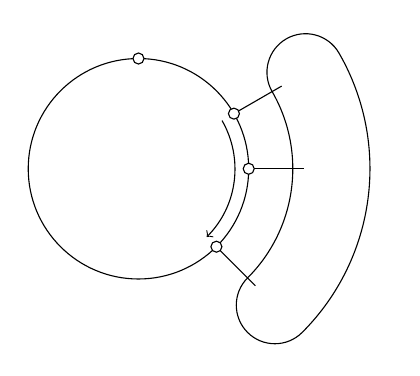
\begin{tikzpicture}[scale=0.7]
      


      \draw (0,0) circle (2cm); \node at (0,0) {};
      \draw (30:2cm) -- (30:3cm); \draw (2,0) -- (3,0); \draw
      (-45:2cm) -- (-45:3cm);
      \node at (38:2.35cm) {}; \node at (2.35,0.25) {}; \node at (-53:2.35cm) {};
      \node at (0,2.35) {};

       \draw (30:2.8cm) arc(30:-45:2.8cm); \draw (30:4.2cm) arc (30:-45:4.2cm);
       \draw (30:2.8cm) arc (-150:-330:0.7cm);
       \draw (-45:2.8cm) arc (135:315:0.7cm);
       \node at (15:3.5cm) {};

       \draw[fill=white] (30:2cm) circle (1mm); \draw[fill=white] (-45:2cm) circle (1mm);
       \draw[fill=white] (2,0) circle (1mm); \draw[fill=white] (0,2) circle (1mm);

       \draw[->] (30:1.75cm) arc (30:-45:1.75cm);
    \end{tikzpicture}
  \end{center}
\caption{ is an earring of , with clasps ; 
  is its first clasp, and  its last clasp. The arrow indicates
  the arc of .}\label{fig:earring}
\end{figure}


\begin{figure}[tbh]
  \begin{center}
    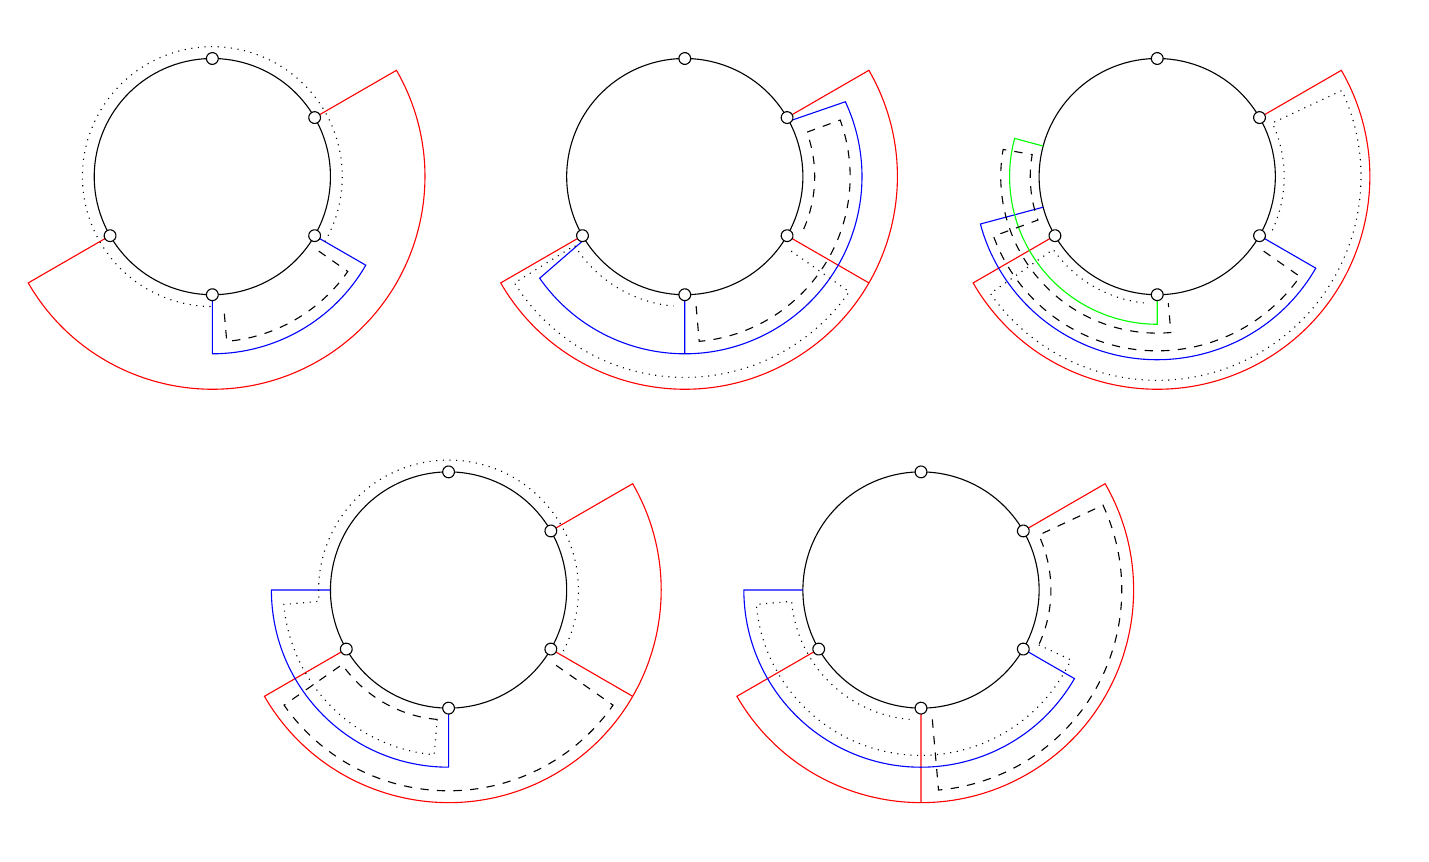
\begin{tikzpicture}[scale=0.75]
      


\begin{scope}[rotate=-60]
        \draw (0,0) circle (2cm); \node at (0,0) {};
        \draw[red] (0,2) -- (0,3.6) arc(90:-90:3.6cm) -- (0,-2);
        \node at (0,1.6) {}; \node at (0,-1.6) {};
        \node at (0,3.9) [font=\footnotesize] {};
        
        \draw[blue] (30:2cm) -- (30:3cm) arc(30:-30:3cm) -- (-30:2cm);
        \node at (30:1.6cm) {}; \node at (-30:1.6cm) {};
        
        \draw[dotted] (30:2.2cm) arc(30:330:2.2cm);
        \draw[dashed] (25:2.2cm) -- (25:2.8cm) arc(25:-25:2.8cm) -- (-25:2.2cm);
        
        \draw[fill=white] (30:2cm) circle (1mm); \draw[fill=white] (-30:2cm) circle (1mm);
        \draw[fill=white] (0,2) circle (1mm); \draw[fill=white] (0,-2) circle (1mm);
        \draw[fill=white] (150:2cm) circle (1mm); \node at (150:1.6cm) {};
      \end{scope}

\begin{scope}[xshift=8cm,rotate=-60]

        \draw (0,0) circle (2cm); \node at (0,0) {};
        \draw[red] (0,2) -- (0,3.6) arc(90:-90:3.6cm) -- (0,-2);
        \node at (0,1.6) {}; \node at (0,-1.6) {};
        \node at (0,3.9) [font=\footnotesize] {};
        \node at (30:1.6cm) {}; \node at (-30:1.6cm) {};

        \draw[red] (30:2cm) -- (30:3.6cm);

        \draw[blue] (88:2cm) -- (85:3cm) arc(85:-85:3cm) -- (-88:2cm);
        \node at (85:3.3cm) [font=\footnotesize] {};
        \draw[blue] (-30:2cm) -- (-30:3cm);

        \draw[dotted] (25:2.2cm) -- (25:3.4cm) arc (25:-88:3.4cm) --
        (-88:2.2cm) arc (-88:-35:2.2cm);
        \draw[dashed] (-25:2.2cm) -- (-25:2.8cm) arc (-25:80:2.8cm) --
        (80:2.2cm) arc (80:35:2.2cm);

        \draw[fill=white] (30:2cm) circle (1mm); \draw[fill=white] (-30:2cm) circle (1mm);
        \draw[fill=white] (0,2) circle (1mm); \draw[fill=white] (0,-2) circle (1mm);
        \draw[fill=white] (150:2cm) circle (1mm); \node at (150:1.6cm) {};
      \end{scope}

\begin{scope}[xshift=16cm,rotate=-60]

        \draw (0,0) circle (2cm); \node at (0,0) {};
        \draw[red] (0,2) -- (0,3.6) arc(90:-90:3.6cm) -- (0,-2);
        \node at (0,1.6) {}; \node at (0,-1.6) {};
        \node at (0,3.9) [font=\footnotesize] {};
        \node at (30:1.6cm) {}; \node at (-30:1.6cm) {};

        \draw[blue] (30:2cm) -- (30:3.1cm) arc (30:-105:3.1cm) -- (-105:2cm);
        \node at (38:2.55cm) [font=\footnotesize] {};
        \draw[green] (-30:2cm) -- (-30:2.5cm) arc(-30:-135:2.5cm) -- (-135:2cm);
        \node at (-143:2.5cm) [font=\footnotesize] {};

        \draw[dotted] (35:2.15cm) arc (35:85:2.15cm) -- (85:3.45cm) arc
        (85:-85:3.45cm) -- (-85:2.15cm) arc (-85:-35:2.15cm);
        \draw[dashed] (25:2.2cm) -- (25:2.95cm) arc(25:-100:2.95cm) --
        (-100:2.15cm) arc (-100:-130:2.15cm) -- (-130:2.65cm) arc
        (-130:-25:2.65cm) -- (-25:2.15cm);

        \draw[fill=white] (30:2cm) circle (1mm); \draw[fill=white] (-30:2cm) circle (1mm);
        \draw[fill=white] (0,2) circle (1mm); \draw[fill=white] (0,-2) circle (1mm);
        \draw[fill=white] (150:2cm) circle (1mm); \node at (150:1.6cm) {};
      \end{scope}

\begin{scope}[xshift=4cm,yshift=-7cm,rotate=-60]

        \draw (0,0) circle (2cm); \node at (0,0) {};
        \draw[red] (0,2) -- (0,3.6) arc(90:-90:3.6cm) -- (0,-2);
        \node at (0,1.6) {}; \node at (0,-1.6) {};
        \node at (0,4.1) [font=\footnotesize] {};
        \node at (30:1.6cm) {}; \node at (-30:1.6cm) {};
        \draw[red] (30:2cm) -- (30:3.6cm);

        \draw[blue] (-30:2cm) -- (-30:3cm) arc(-30:-120:3cm) -- (-120:2cm);
        \node at (-125:3cm) [font=\footnotesize] {};
        
        \draw[dashed] (-35:2.2cm) arc (-35:-85:2.2cm) -- (-85:3.4cm)
        arc (-85:25:3.4cm) -- (25:2.2cm);
        \draw[dotted] (-35:2.2cm) -- (-35:2.8cm) arc(-35:-115:2.8cm)
        -- (-115:2.2cm) arc (-115:-330:2.2cm);

        \draw[fill=white] (30:2cm) circle (1mm); \draw[fill=white] (-30:2cm) circle (1mm);
        \draw[fill=white] (0,2) circle (1mm); \draw[fill=white] (0,-2) circle (1mm);
        \draw[fill=white] (150:2cm) circle (1mm); \node at (150:1.6cm) {};
      \end{scope}

\begin{scope}[xshift=12cm,yshift=-7cm,rotate=-60]

        \draw (0,0) circle (2cm); \node at (0,0) {};
        \draw[red] (0,2) -- (0,3.6) arc(90:-90:3.6cm) -- (0,-2);
        \node at (0,1.6) {}; \node at (0,-1.6) {};
        \node at (0,4.1) [font=\footnotesize] {};
        \node at (30:1.6cm) {}; \node at (-30:1.6cm) {};
        \draw[red] (-30:2cm) -- (-30:3.6cm);

        \draw[blue] (30:2cm) -- (30:3cm) arc(30:-120:3cm) -- (-120:2cm);
        \node at (-125:3cm) [font=\footnotesize] {};
        
        \draw[dashed] (-25:2.2cm) -- (-25:3.4cm) arc (-25:85:3.4cm) -- (85:2.2cm)
        arc (85:35:2.2cm);
        \draw[dotted] (-35:2.2cm) arc (-35:-115:2.2cm) -- (-115:2.8cm) arc(-115:35:2.8cm)
        -- (35:2.2cm);

        \draw[fill=white] (30:2cm) circle (1mm); \draw[fill=white] (-30:2cm) circle (1mm);
        \draw[fill=white] (0,2) circle (1mm); \draw[fill=white] (0,-2) circle (1mm);
        \draw[fill=white] (150:2cm) circle (1mm); \node at (150:1.6cm) {};
      \end{scope}

    \end{tikzpicture}
  \end{center}
  \caption{The various cases of Theorem~\ref{thm:earringProof} are
    illustrated in the order presented. In each case, one of the 2
    vertex-disjoint paths from  to  is indicated with dashed
    lines, and the other with dotted lines.}\label{fig:earringProof}
\end{figure}

\begin{theorem}\label{thm:earringProof}
Let  be an earring of minimum arc length. Every segment contained
in the arc of  is safe.
\end{theorem}
\begin{proof}
  Let  be the set of earrings with arc identical to that
  of . Since they have the same arc, we refer to this as the arc of
  , or the \emph{critical arc}. Let the first clasp of
  every earring in  be , and the last clasp of each
  earring in  be . Because the earrings in
   have arcs of minimum length, any earring  has a clasp  that is not in the critical arc. (That
  is,  or .)

  We must show that every segment contained in the critical arc is
  safe; recall that a segment  is safe if the graph  is
  2-connected.  Given an arbitrary segment  in the critical arc,
  let  and  () be the anchors that are its
  endpoints. We prove that there are always 2 internally
  vertex-disjoint paths between  and  in ; this
  suffices to show 2-connectivity.

  We consider several cases, depending on the earrings that contain
   and . Figure~\ref{fig:earringProof} illustrates these
  cases.  If  and  are contained in the same earring ,
  it is easy to find two vertex-disjoint paths between them in
  . The first path is clockwise from  to  in the cycle
  . The second path is entirely contained in the earring  (an
  earring is connected in , so we can always find such a path.)

  Otherwise,  and  are clasps of distinct earrings. We
  consider three cases: Both  and  are clasps of earrings in
  , one is (but not both), or neither is.
  \begin{enumerate}
  \item We first consider that both  and  are clasps of
    earrings in . Let  be a clasp of , and 
    a clasp of . The first path is from  to  through
    , and then clockwise along the critical arc from  to
    . The second path is from  to  clockwise along the
    critical path, and then  to  through . It is easy
    to see that these paths are internally vertex-disjoint.

  \item Now, suppose neither  nor  is a clasp of an earring
    in . Let  be a clasp of , and  be a
    clasp of . The first path we find follows the critical arc
    clockwise from  to  (the last clasp of the critical
    arc), from  to  through , and again
    clockwise through the critical arc from  to . Internal
    vertices of this path are all in  or on the critical arc. Let
     be a clasp of  not on the critical arc, and 
    be a last clasp of  not on the critical arc. The second path
    goes from  to  through , from  to 
    through the cycle  outside the critical arc, and from 
    to  through . Internal vertices of this path are in
    , or in , but not part of the critical arc (since
    each of  and  are outside the critical arc).
    Therefore, we have 2 vertex-disjoint paths from  to .


  \item Finally, we consider the case that exactly one of 
    is a clasp of an earring in . Suppose  is a clasp
    of , and  is a clasp of ; the other case (where  and
     is symmetric, and omitted, though
    figure~\ref{fig:earringProof} illustrates the paths.) Let  be
    the index of a clasp of  outside the critical arc. The first
    path is from  to  through the critical arc, and then
    from  to  through . The second path is from 
    to  through , and from  to  clockwise
    through . Note that the last part of this path enters the
    critical arc at , and continues through the arc until .
    Internal vertices of the first path that are in  are on the
    critical arc, but have index greater than . Internal vertices
    of the second path that belong to  are either not in the
    critical arc, or have index between  and . Therefore,
    the two paths are internally vertex-disjoint. \qedhere
  \end{enumerate}
\end{proof}

We now describe our algorithm to find a non-trivial cycle of good
density, proving Theorem~\ref{thm:cycle}:
  \emph{Let  be a -connected graph with edge-costs and terminal weights,
  and at least  terminals. There is a polynomial-time algorithm to
  find a non-trivial cycle  in  such that .}

\begin{proofof}{Theorem~\ref{thm:cycle}}
  Let  be a graph with  terminals and density ; we describe
  a polynomial-time algorithm that either finds a cycle in  of density
  less than , or a proper subgraph  of  that contains all 
  terminals. In the latter case, we can recurse on  until we eventually
  find a cycle of density at most .

  We first find, in  time, a minimum-density cycle  in . By
  Theorem~\ref{thm:cycleExists},  has density at most , because
  the minimum-density \emph{non-trivial} cycle has at most this density.
  If  contains at least 2 terminals, we are done. Otherwise, 
  contains exactly one terminal . Since  contains at least 2
  terminals, there must exist at least one earring of .

  Let  be the origin of this cycle , and  an earring of minimum
  arc length. By Theorem~\ref{thm:earringProof}, every segment in the arc
  of  is safe. Let  be such a segment; since  was selected as the
  origin,  is not an internal vertex of . As  is the only terminal
  of ,  contains no terminals, and therefore, the graph 
  is 2-connected, and contains all  terminals of .
\end{proofof}

The proof above also shows that if  is minimally 2-connected on its
terminals (that is,  has no 2-connected proper subgraph containing
all its terminals), every cycle of  is non-trivial. (If a cycle
contains 0 or 1 terminals, it has a safe segment containing no
terminals, which can be deleted; this gives a contradiction.)
Therefore, given a graph that \emph{is} minimally 2-connected on its
terminals, finding a minimum-density non-trivial cycle is equivalent
to finding a minimum-density cycle, and so can be solved exactly in
polynomial time.  This suggests a natural algorithm for the problem:
Given a graph that is not minimally 2-connected on its terminals,
delete edges and vertices until the graph is minimally 2-connected on
the terminals, and then find a minimum-density cycle. As shown above,
this gives a cycle of density no more than that of the input graph,
but this may not be the minimum-density cycle of the original
graph. For instance, there exist instances where the minimum-density
cycle uses edges of a safe segment  that might be deleted by this
algorithm.


\section{Pruning 2-connected Graphs of Good Density}
\label{sec:pruning}

In this section, we prove Theorem~\ref{thm:avekv}. We are given a
graph  and , a set of at least  terminals.
Further, every terminal in  has 2 vertex-disjoint paths to the root
 of total cost at most . Let  be the number of terminals
in , and  its total cost;  is
the density of . We describe an algorithm that finds a subgraph 
of  that contains at least  terminals, each of which is
2-connected to the root, and of total edge cost .

We can assume , or the trivial solution of
taking the entire graph  suffices. The main phase of our algorithm
proceeds by maintaining a set of 2-connected subgraphs that we call
\emph{clusters}, and repeatedly finding low-density cycles that merge
clusters of similar weight to form larger clusters.  (The weight of a
cluster , denoted by , is (roughly) the number of terminals it
contains.) Clusters are grouped into \emph{tiers} by weight; tier 
contains clusters with weight at least  and less than
. Initially, each terminal is a separate cluster in tier
0. We say a cluster is \emph{large} if it has weight at least , and
\emph{small} otherwise. The algorithm stops when most terminals are in
large clusters.

We now describe the algorithm {\sc MergeClusters} (see next page). To simplify
notation, let  be the quantity .  We say
that a cycle is \emph{good} if it has density at most ; that
is, good cycles have density at most  times the density of
the input graph.

\begin{algo}
\underline{\sc MergeClusters}:\\
For (each  in ) do: \+ \\
    If (): \+ \\
        Every terminal has weight 1 \- \\
    Else: \+ \\
        Mark all vertices as non-terminals \\
        For (each small 2-connected cluster  in tier ) do: \+ \\
             Add a (dummy) terminal  to  of weight  \\
             Add (dummy) edges of cost 0 from  to two (arbitrary) distinct vertices of  \- \- \\

    While ( has a non-trivial cycle  of density at most  in ): \+ \\
        Let  be the small clusters that contain a terminal
           {\bf or an edge} of .\\
        (Note that the terminals in  belong to a subset of .)\\
        Form a new cluster  (of a higher tier) by merging the clusters \\
         \\
        If (): \+ \\
            Mark all terminals in  as non-terminals \- \\
        Else: \+ \\
            Delete all (dummy) terminals in  and the associated (dummy) edges.
\end{algo}

We briefly remark on some salient features of this algorithm and our
analysis before presenting the details of the proofs.
\begin{enumerate}
\item In iteration , the terminals correspond to tier 
  clusters. Clusters are 2-connected subgraphs of , and by using
  cycles to merge clusters, we preserve 2-connectivity as the clusters
  become larger.

\item When a cycle  is used to merge clusters, all small clusters
  that contain an edge of  (regardless of their tier) are merged to
  form the new cluster. Therefore, at any stage of the algorithm, all
  currently small clusters are edge-disjoint.  Large clusters, on the
  other hand, are \emph{frozen}; even if they intersect a good cycle
  , they are not merged with other clusters on . Thus, at any
  time, an edge may be in multiple large clusters and up to one small
  cluster.

\item In iteration  of {\sc MergeClusters}, the density of a cycle
   is only determined by its cost and the weight of terminals in
   corresponding to tier  clusters. Though small clusters of
  other (lower or higher) tiers might be merged using , we do
  \emph{not} use their weight to pay for the edges of .

\item The th iteration terminates when no good cycles can be found
  using the remaining tier  clusters. At this point, there may be
  some terminals remaining that correspond to clusters which are not
  merged to form clusters of higher tiers. However, our choice of
   (which defines the density of good cycles) is such that we
  can bound the number of terminals that are ``left behind'' in this
  fashion. Therefore, when the algorithm terminates, most terminals
  are in large clusters.
\end{enumerate}

By bounding the density of large clusters, we can find a solution to
the rooted \kv problem of bounded density. Because we always use
cycles of low density to merge clusters, an analysis similar to that
of \cite{LauNSS07} and \cite{ChekuriKP08} shows that every large
cluster has density at most . We first present this
analysis, though it does not suffice to prove Theorem~\ref{thm:avekv}.
A more careful analysis shows that there is at least one large cluster
of density at most ; this allows us to prove the
desired theorem.

We now formally prove that {\sc MergeClusters} has the desired
behavior. First, we present a series of claims which, together, show
that when the algorithm terminates, most terminals are in large
clusters, and all clusters are 2-connected.

\begin{remark}\label{rem:cluster}
  Throughout the algorithm, the graph  is always 2-connected. The
  weight of a cluster is at most the number of terminals it contains.
\end{remark}
\begin{proof}
  The only structural changes to  are when new vertices are added
  as terminals; they are added with edges to two distinct vertices of
  . This preserves 2-connectivity, as does deleting these terminals
  with the associated edges.

  To see that the second claim is true, observe that if a terminal
  contributes weight to a cluster, it is contained in that cluster. A
  terminal can be in multiple clusters, but it contributes to the
  weight of exactly one cluster.
\end{proof}

We use the following simple proposition in proofs of 2-connectivity;
the proof is straightforward, and hence omitted.

\begin{proposition}\label{prop:shareEdge}
  Let  and  be -connected subgraphs
  of a graph  such that .  Then the
  graph  is
  -connected.
\end{proposition}

\begin{lemma}\label{lem:clusters2conn}
The clusters formed by {\sc MergeClusters} are all -connected.
\end{lemma}
\begin{proof}
  Let  be a cluster formed by using a cycle  to merge clusters
  . The edges of the cycle  form a
  2-connected subgraph of , and we assume that each  is
  2-connected by induction.  Further,  contains at least 2 vertices
  of each \footnote{A cluster  may be a singleton vertex
    (for instance, if we are in tier 0), but such a vertex does not
    affect 2-connectivity.}, so we can use induction and
  Proposition~\ref{prop:shareEdge} above: We assume  is 2-connected by induction, and  contains 2
  vertices of , so  is
  2-connected.

  Note that we have shown  is 2-connected,
  but  (and hence ) might contain dummy terminals and the
  corresponding dummy edges. However, each such terminal with the 2
  associated edges is a ear of ; deleting them leaves 
  2-connected.
\end{proof}

\begin{lemma}\label{lem:fewLeftBehind}
  The total weight of small clusters in tier  that are not merged to form
  clusters of higher tiers is at most .
\end{lemma}
\begin{proof}
  Assume this were not true; this means that {\sc MergeClusters} could
  find no more cycles of density at most  using the remaining
  small tier  clusters.  But the total cost of all the edges is at
  most , and the sum of terminal weights is at least
  ; this implies that the density of the
  graph (using the remaining terminals) is at most . But by
  Theorem~\ref{thm:cycleExists}, the graph must then contain a good
  non-trivial cycle, and so the while loop would not have terminated.
\end{proof}

\begin{corollary}\label{cor:weightLargeClusters}
  When the algorithm {\sc MergeClusters} terminates, the total weight of large
  clusters is at least .
\end{corollary}
\begin{proof}
  Each terminal not in a large cluster contributes to the weight of a
  cluster that was not merged with others to form a cluster of a
  higher tier. The previous lemma shows that the total weight of such
  clusters in any tier is at most ;
  since there are  tiers, the total number of terminals
  not in large clusters is less than .
\end{proof}


So far, we have shown that most terminals reach large clusters, all of
which are 2-connected, but we have not argued about the density of
these clusters. The next lemma says that if we can find a large
cluster of good density, we can find a solution to the \kv problem of
good density.

\begin{lemma}\label{lem:segment}
  Let  be a large cluster formed by {\sc MergeClusters}. If  has
  density at most , we can find a graph  with at least 
  terminals, each of which is -connected to , of total cost at
  most .
\end{lemma}
\begin{proof}
  Let  be the clusters merged to form  in
  order around the cycle  that merged them; each  was a small
  cluster, of weight at most . A simple averaging argument shows
  that there is a consecutive segment of s with total weight
  between  and , such that the cost of the edges of 
  connecting these clusters, together with the costs of the clusters
  themselves, is at most . Let  be the ``first''
  cluster of this segment, and  the ``last''. Let  and  be
  arbitrary terminals of  and  respectively. Connect each of
   and  to the root  using 2 vertex-disjoint paths; the cost
  of this step is at most . (We assumed that every terminal could
  be 2-connected to  using disjoint paths of cost at most .)
  The graph  thus constructed has at least  terminals, and
  total cost at most .  

  We show that every vertex  of  is 2-connected to ; this
  completes our proof. Let  be an arbitrary vertex of ; suppose
  there is a cut-vertex  which, when deleted, separates  from
  . Both  and  are 2-connected to , and therefore neither
  is in the same component as  in . However, we describe 2
  vertex-disjoint paths  and  in  from  to  and
   respectively; deleting  cannot separate  from both  and
  , which gives a contradiction. The paths  and  are easy
  to find; let  be the cluster containing . The cycle 
  contains a path from vertex  to , and
  another (vertex-disjoint) path from  to .
  Concatenating these paths with paths from  to  in  and
   to  in  gives us vertex-disjoint paths  from 
  to  and  from  to . Since  is 2-connected, we
  can find vertex-disjoint paths from  to  and , which
  gives us the desired paths  and .\footnote{The vertex 
    may not be in any cluster . In this case,  is formed by
    using edges of  from  to , and then a path from
     to ;  is formed similarly.}
\end{proof}

\bigskip
We now present the two analyses of density referred to earlier. The
key difference between the weaker and tighter analysis is in the way
we bound edge costs. In the former, each large cluster pays for its
edges separately, using the fact that all cycles used have density at
most . In the latter, we crucially use the fact
that small clusters which share edges are merged. Roughly speaking,
because small clusters are edge-disjoint, the average density of small
clusters must be comparable to the density of the input graph
. Once an edge is in a large cluster, we can no longer use the
edge-disjointness argument. We must pay for these edges separately,
but we can bound this cost.

First, the following lemma allows us to show that every large cluster
has density at most .

\begin{lemma} \label{lem:tierCost}
  For any cluster  formed by {\sc MergeClusters} during iteration ,
  the total cost of edges in  is at most .
\end{lemma}
\begin{proof}
  We prove this lemma by induction on the number of vertices in a
  cluster.  Let  be the set of clusters merged using a
  cycle  to form .  Let  be the set of clusters in
   of tier , and  be . ( contains clusters of tiers less or
  greater than  that contained an edge of .)

  The cost of edges in  is at most the sum of: the cost of , the
  cost of , and the cost of . Since all
  clusters in  have been formed during iteration  or
  earlier, and are smaller than , we can use induction to show that
  the cost of edges in  is at most . All clusters in  are of tier
  , and so must have been formed before iteration  (any cluster
  formed during iteration  is of a strictly greater tier), so we
  use induction to bound the cost of edges in  by .

  Finally, because  was a good-density cycle, and only clusters of
  tier  contribute to calculating the density of , the cost of
   is at most . Therefore,
  the total cost of edges in  is at most .
\end{proof}

\bigskip
Let  be an arbitrary large cluster; since we have only 
tiers, the previous lemma implies that the cost of  is at most
. That is, the
density of  is at most , and we can use this fact
together with Lemma~\ref{lem:segment} to find a solution to the rooted \kv
problem of cost at most . This completes the
`weaker' analysis, but this does not suffice to prove
Theorem~\ref{thm:avekv}; to prove the theorem, we would need to use a large
cluster  of density , instead of .

For the purpose of the more careful analysis, implicitly construct a
forest  on the clusters formed by {\sc
  MergeClusters}. Initially, the vertex set of  is just
, the set of terminals, and  has no edges. Every time a
cluster  is formed by merging  , we add a
corresponding vertex  to the forest , and add edges
from  to each of ;  is the parent of . We also associate a cost with each vertex in
; the cost of the vertex  is the cost of the cycle used
to form  from . We thus build up trees as the
algorithm proceeds; the root of any tree corresponds to a cluster that
has not yet become part of a bigger cluster. The leaves of the trees
correspond to vertices of ; they all have cost 0. Also, any large
cluster  formed by the algorithm is at the root of its tree; we
refer to this tree as .

For each large cluster  after {\sc MergeClusters} terminates, say
that  is of type  if  was formed during iteration  of
MergeClusters. We now define the \emph{final-stage} clusters of :
They are the clusters formed during iteration  that became part of
. (We include  itself in the list of final-stage clusters; even
though  was formed in iteration  of {\sc MergeClusters}, it may
contain other final-stage clusters. For instance, during iteration
, we may merge several tier  clusters to form a cluster  of
tier . Then, if we find a good-density cycle  that contains
an edge of ,  will merge with the other clusters of .)  The
\emph{penultimate} clusters of  are those clusters that exist just
before the beginning of iteration  and become a part of
. Equivalently, the penultimate clusters are those formed before
iteration  that are the immediate children in  of final-stage
clusters. Figure 1 illustrates the definitions of final-stage and
penultimate clusters. Such a tree could be formed if, in iteration
, 4 clusters of this tier merged to form , a cluster of tier
. Subsequently, in iteration , clusters  and  merge to
form . We next find a good cycle containing  and ; 
contains an edge of this cycle, so these three clusters are merged to
form . Note that the cost of this cycle is paid for the by the
weights of  and  only;  is a tier  cluster, and so its
weight is not included in the density calculation. Finally, we find a
good cycle paid for by  and ; since  and  share edges with
this cycle, they all merge to form the large cluster .

\begin{figure}[tbh]
  \begin{center}
  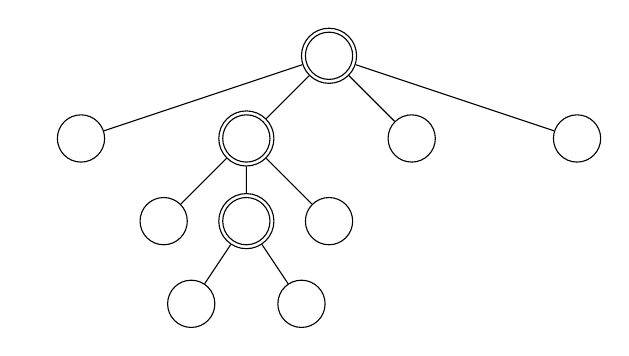
\begin{tikzpicture}[scale=0.7]
    \tikzstyle{vertex}=[circle,draw,inner sep=0pt,minimum size=6mm];
    \tikzstyle{high}=[circle,draw,inner sep=0pt,minimum size=7mm];

    \tikzstyle{every node}=[font=\tiny];

\node (y) at (6,5.5) [high] {};

\node (a) at (1.5,4) [vertex] {}; \node (b) at (4.5,4) [high] {};
    \node (c) at (7.5,4) [vertex] {}; \node (d) at (10.5,4) [vertex] {}; 
    \draw (a) -- (y) -- (b); \draw (c) -- (y) -- (d);

    \node at (0.7,4) {}; \node at (3.6,4) {}; \node at (6.7,4) {};
    \node at (9.7,4) {};



\node (e) at (3,2.5) [vertex] {}; \node (f) at (4.5,2.5) [high] {};
    \node (g) at (6,2.5) [vertex] {};
    \draw (e) -- (b) -- (f); \draw (b) -- (g);

    \node at (2.3,2.7) {}; \node at (3.8,2.7) {}; \node at (5.35,2.7) {};

    \node (h) at (3.5,1) [vertex] {}; \node (j) at (5.5,1) [vertex] {};
    \draw (h) -- (f) -- (j); 

    \node at (2.9,1.3) {}; \node at (4.9,1.3) {}; 









    \node at (y) [vertex] {}; \node at (b) [vertex] {}; \node at (f) [vertex] {};

  \end{tikzpicture}
  \end{center}
  \caption{A part of the Tree  corresponding to , a large
    cluster of type . The number in each vertex indicates the tier
    of the corresponding cluster.  Only final-stage and penultimate
    clusters are shown: final-stage clusters are indicated with a
    double circle; all other clusters are penultimate.}
\end{figure}

An edge of a large cluster  is said to be a \emph{final edge} if it
is used in a cycle  that produces a final-stage cluster of . All
other edges of  are called \emph{penultimate edges}; note that any
penultimate edge is in some penultimate cluster of . We define the
\emph{final cost} of  to be the sum of the costs of its final
edges, and its \emph{penultimate cost} to be the sum of the costs of
its penultimate edges; clearly, the cost of  is the sum of its
final and penultimate costs. We bound the final costs and penultimate
costs separately.

Recall that an edge is a final edge of a large cluster  if it is
used by {\sc MergeClusters} to form a cycle  in the final iteration
during which  is formed. The reason we can bound the cost of final
edges is that the cost of any such cycle is at most  times the
weight of clusters contained in the cycle, and a cluster does not
contribute to the weight of more than one cycle in an iteration. (This
is also the essence of Lemma~\ref{lem:tierCost}.) We formalize this
intuition in the next lemma.

\begin{lemma}\label{lem:final}
  The final cost of any large cluster  is at most ,
  where  is the weight of .
\end{lemma}
\begin{proof}
  Let  be an arbitrary large cluster. In the construction of the
  tree , we associated with each vertex of  the cost of the
  cycle used to form the corresponding cluster. To bound the total
  final cost of , we must bound the sum of the costs of vertices of
   associated with final-stage clusters.  The weight of ,
   is at least the sum of the weights of the penultimate tier 
  clusters that become a part of . Therefore, it suffices to show
  that the sum of the costs of vertices of  associated with
  final-stage clusters is at most  times the sum of the
  weights of 's penultimate tier  clusters. (Note that a tier
   cluster must have been formed prior to iteration , and hence
  it cannot itself be a final-stage cluster.)

  A cycle was used to construct a final-stage cluster  only if its
  cost was at most  times the sum of weights of the
  penultimate tier  clusters that become a part of . (Larger
  clusters may become a part of , but they do not contribute weight
  to the density calculation.)  Therefore, if  is a vertex of 
  corresponding to a final-stage cluster, the cost of  is at most
   times the sum of the weights of its tier  immediate
  children in . But  is a tree, and so no vertex
  corresponding to an penultimate tier  cluster has more than one
  parent. That is, the weight of a penultimate cluster pays for only
  one final-stage cluster. Therefore, the sum of the costs of vertices
  associated with final-stage clusters is at most  times the
  sum of the weights of 's penultimate tier  clusters, and so
  the final cost of  is at most .
\end{proof}


\begin{lemma}\label{lem:penultimate}
  If  and  are distinct large clusters of the same type, no
  edge is a penultimate edge of both  and .
\end{lemma}
\begin{proof}
  Suppose, by way of contradiction, that some edge  is a
  penultimate edge of both  and , which are large clusters
  of type . Let  (respectively ) be a penultimate cluster
  of  (resp. ) containing . As penultimate clusters, both
   and  are formed before iteration . But until iteration
  , neither is part of a large cluster, and two small clusters
  cannot share an edge without being merged. Therefore,  and
   must have been merged, so they cannot belong to distinct large
  clusters, giving the desired contradiction.
\end{proof}

\begin{theorem}\label{thm:goodLargeCluster}
  After {\sc MergeClusters} terminates, at least one large cluster has
  density at most .
\end{theorem}
\begin{proof}
  We define the \emph{penultimate density} of a large cluster to be
  the ratio of its penultimate cost to its weight.

  Consider the total penultimate costs of all large clusters: For any
  , each edge  can be a penultimate edge of at most 1
  large cluster of type . This implies that each edge can be a
  penultimate edge of at most  clusters. Therefore, the
  sum of penultimate costs of all large clusters is at most
  . Further, the total weight of all large
  clusters is at least .  Therefore, the (weighted) average
  penultimate density of large clusters is at most , and hence there exists a
  large cluster  of penultimate density at most .

  The penultimate cost of  is, therefore, at most , and from Lemma~\ref{lem:final}, the final cost of 
  is at most .  Therefore, the density of  is at most
  .
\end{proof}

Theorem~\ref{thm:goodLargeCluster} and Lemma \ref{lem:segment}
together imply that we can find a solution to the rooted \kv problem
of cost at most . This completes our proof of
Theorem~\ref{thm:avekv}.



\section{Conclusions}
\label{sec:conclusion}

We list the following open problems:
\begin{itemize}
\item Can the approximation ratio for the \kv problem be improved from
  the current  to  or better? Removing
  the dependence on  to obtain even  could be
  interesting. If not, can one improve the approximation ratio for the
  easier \ke problem?

\item Can we obtain approximation algorithms for the \kvc{\lambda} or
  \kec{\lambda} problems for ? In general, few results
  are known for problems where vertex-connectivity is required to be
  greater than 2, but there has been more progress with higher
  edge-connectivity requirements.

\item Given a 2-connected graph of density  with some vertices
  marked as terminals, we show that it contains a non-trivial cycle
  with density at most , and give an algorithm to find such a
  cycle. We have also found an -approximation for the
  problem of finding a minimum-density non-trivial cycle. Is there a
  constant-factor approximation for this problem? Can it be solved
  \emph{exactly} in polynomial time?
\end{itemize}

\medskip
\noindent
\textbf{Acknowledgments:} We thank Mohammad Salavatipour for helpful
discussions on \ke and related problems. We thank Erin Wolf Chambers
for useful suggestions on notation.


\bibliographystyle{plain}

\begin{thebibliography}{99}
\bibitem{AgrawalKR95}
A.~Agrawal, P.~N. Klein, and R.~Ravi.
\newblock When trees collide: An Approximation Algorithm for the Generalized
  {S}teiner Problem on Networks.
\newblock {\em SIAM J. on Computing}, 24(3):440--456, 1995.

\bibitem{networkflows_book}
R.~Ahuja, T.~Magnanti, and J.~Orlin.
\newblock Network Flows: Theory, Algorithms, and Applications.
\newblock Prentice Hall, Upper Saddle River, NJ, 1993

\bibitem{AwerbuchABV95}
B. Awerbuch, Y. Azar, A. Blum and S. Vempala.
\newblock  New Approximation Guarantees for Minimum Weight -Trees and 
Prize-Collecting Salesmen.
\newblock {\em SIAM J.\ on Computing}, 28(1):254--262, 1999. Preliminary
version in {\em Proc.\ of ACM STOC}, 1995.

\bibitem{orienteering}
A.~Blum, S.~Chawla, D.~Karger, T.~Lane, A.~Meyerson, and M.~Minkoff.
\newblock Approximation Algorithms for Orienteering and Discounted-Reward TSP.
\newblock {\em SIAM J.\ on Computing}, 37(2):653--670, 2007.

\bibitem{BlumRV96}
A. Blum, R. Ravi and S. Vempala.
\newblock  A Constant-factor Approximation Algorithm for the -MST Problem.
\newblock {\em JCSS}, 58:101--108, 1999.
\newblock Preliminary version in {\em Proc.\ of ACM STOC}, 1996.

\bibitem{ChaudhuriGRT03}
K.~Chaudhuri, B.~Godfrey, S.~Rao, and K.~Talwar.
\newblock Paths, trees, and minimum latency tours.
\newblock {\em Proc.\ of IEEE FOCS}, 36--45, 2003.

\bibitem{ChekuriEGS08}
C.~Chekuri, G.~Even, A.~Gupta, and D. Segev.
\newblock Set Connectivity Problems in Undirected Graphs and the 
Directed Steiner Network Problem.
\newblock {\em Proc.\ of ACM-SIAM SODA}, 532--541, 2008.

\bibitem{ChekuriHKS06}
C.~Chekuri, M.~T. Hajiaghayi, G.~Kortsarz, and M.~R. Salavatipour.
\newblock Approximation algorithms for Non-uniform Buy-at-bulk Network Design.
\newblock {\em Proc. of IEEE FOCS}, 677--686, 2006.

\bibitem{ChekuriHKS07}
C.~Chekuri, M.~T. Hajiaghayi, G.~Kortsarz, and M.~R. Salavatipour.
\newblock Approximation Algorithms for Node-weighted Buy-at-bulk Network
  Design.
\newblock {\em Proc. of ACM-SIAM SODA}, 1265--1274, 2007.

\bibitem{ChekuriKP08}
C.~Chekuri, N.~Korula, and M.~P\'{a}l.
\newblock Improved Algorithms for Orienteering and Related Problems.
\newblock {\em Proc. of ACM-SIAM SODA}, 661--670, 2008.

\bibitem{ChudakRW}
F.~A. Chudak, T.~Roughgarden, and D.~P. Williamson.
\newblock Approximate -MSTs and -Steiner Trees via the Primal-Dual
Method and Lagrangean Relaxation.
\newblock {\em Proc. of IPCO}, 60--70, 2001.

\bibitem{FeigeKP01}
U. Feige, G. Kortsarz and D. Peleg.
\newblock The Dense -Subgraph Problem.
\newblock {\em Algorithmica}, 29(3):410--421, 2001.
\newblock Preliminary version in {\em Proc.\ of IEEE FOCS}, 1993.

\bibitem{FleischerJW}
L. Fleischer, K. Jain, D.~P. Williamson.
\newblock Iterative Rounding 2-approximation Algorithms for Minimum-cost Vertex
Connectivity Problems.
\newblock {\em J. of Computer and System Sciences}, 72(5):838--867, 2006.

\bibitem{Garg05}
N. Garg.
\newblock Saving an : A -approximation for the -MST Problem in 
Graphs.
\newblock {\em Proc.\ of ACM STOC}, 396--402, 2005.

\bibitem{Garg96}
N.~Garg.
\newblock A 3-approximation for the Minimum Tree Spanning  Vertices.
\newblock {\em Proc.\ of IEEE FOCS}, 302--309, 1996.

\bibitem{GoemansW95}
M.~X. Goemans and D.~P. Williamson.
\newblock A General Approximation Technique for Constrained Forest Problems.
\newblock {\em SIAM J. on Computing}, 24(2):296--317, 1995.

\bibitem{GoemansW96}
M.~X. Goemans and D.~P. Williamson.
\newblock The Primal-Dual method for Approximation Algorithms and its
  Application to Network Design Problems.
\newblock In D.~S. Hochbaum, editor, {\em Approximation Algorithms for NP-Hard
  Problems}. PWS Publishing Company, 1996.

\bibitem{HajiaghayiJ}
M.~T. Hajiaghayi and K.~Jain.
\newblock The Prize-Collecting Generalized Steiner Tree Problem via a New
Approach of Primal-Dual Schema.
\newblock {\em Proc of ACM-SIAM SODA}, 631--640, 2006.

\bibitem{Hochbaum96}
D.~S. Hochbaum, editor.
\newblock {\em Approximation Algorithms for NP-Hard Problems}.
\newblock PWS Publishing Company, 1996.

\bibitem{Jain}
K. Jain.
\newblock{A Factor 2 Approximation Algorithm for the Generalized Steiner Network
  Problem}
\newblock {\em Combinatorica}, 21(1):39--60, 2001.
Preliminary version in {\em Proc.\ of IEEE FOCS}, 448--457, 1998.

\bibitem{Johnson74}
D.~S. Johnson.
\newblock Approximation Algorithms for Combinatorial Problems.
\newblock {\em J. of Computer and System Sciences}, 9(3):256--278, 1974.

\bibitem{LauNSS07}
L.C. Lau, J. Naor, M. Salavatipour and M. Singh.
\newblock Survivable Network Design with Degree or Order Constraints.
\newblock {\em Proc.\ of ACM STOC}, 2007.

\bibitem{LauNSS07b}
L.C. Lau, J. Naor, M. Salavatipour and M. Singh.
\newblock Survivable Network Design with Degree or Order Constraints.
\newblock Manuscript, 2007.


\bibitem{Seymour}
P.~D. Seymour.
\newblock Nowhere-zero 6-flows
\newblock {\em J. Comb. Theory B}, 30: 130--135, 1981.

\bibitem{Vazirani01}
V.~V. Vazirani.
\newblock {\em Approximation Algorithms}.
\newblock Springer, 2001.

\end{thebibliography}

\end{document}